\documentclass[aspectratio=169,11pt,t]{beamer}
% ============================================================
%  ksa-cs-v2: ksa-cs-lecture-template.tex 스타일 + 한글, v2 덱(16:9)용.
%    - 짙은 네이비 헤드라인 (섹션 이름 + 프레임마다 점)
%    - 꽉 찬 파란 제목 막대, 둥근 그림자 블록
%    - 한글: Noto Sans CJK KR (fontspec)
%  사용:
%    \documentclass[aspectratio=169,11pt,t]{beamer}
%    \input{<..>/theme/ksa-cs-v2.tex}
%  ksa-theme.tex 의 매크로(\kb \kq, ksablue/ksared 등)도 같은 이름으로 둔다
%  -> v2 덱 본문을 거의 그대로 옮길 수 있다.
% ============================================================

\usepackage{fontspec}
\usepackage{amsmath,amssymb}
\usepackage{tikz}
\usepackage{listings}
\usepackage{graphicx}
\usepackage{booktabs}
\usepackage{varwidth}
% enumitem 은 넣지 않는다 (beamer 글머리표가 사라진다)

\defaultfontfeatures{Ligatures=TeX}
\setmainfont{Noto Sans CJK KR}
\setsansfont{Noto Sans CJK KR}
\setmonofont{Noto Sans Mono CJK KR}[Scale=0.92]
\usefonttheme{professionalfonts}

% ---------- 기본 틀 ----------
\usetheme{default}
\useinnertheme[shadow=true]{rounded}
\setbeamertemplate{navigation symbols}{}
\setbeamersize{text margin left=1em,text margin right=1em}

% ---------- 색 (템플릿 원본 값) ----------
\definecolor{navydark}{HTML}{191959}
\definecolor{navydim}{HTML}{8888B0}
\definecolor{navytitle}{HTML}{262686}
\definecolor{navyblue}{HTML}{3333B2}
\definecolor{blockbodybg}{HTML}{E9E9F3}
\definecolor{examplegreen}{HTML}{006000}
\definecolor{examplebg}{HTML}{E5EFE5}
\definecolor{alertred}{HTML}{BF0000}
\definecolor{alertbg}{HTML}{F9E5E5}
% ksa-theme.tex 와 같은 이름 (본문 호환)
\colorlet{ksablue}{navytitle}
\colorlet{ksabluedk}{navydark}
\definecolor{ksagold}{HTML}{D6CBB1}
\definecolor{ksagolddk}{HTML}{A9976B}
\colorlet{ksared}{alertred}
\definecolor{ksagray}{HTML}{5B5B5B}

\setbeamercolor{structure}{fg=navyblue}
\setbeamercolor{alerted text}{fg=alertred}
\setbeamercolor{frametitle}{bg=navytitle,fg=white}
\setbeamercolor{title}{fg=white,bg=navytitle}
\setbeamercolor{block title}{bg=navytitle,fg=white}
\setbeamercolor{block body}{bg=blockbodybg,fg=black}
\setbeamercolor{block title example}{bg=examplegreen,fg=white}
\setbeamercolor{block body example}{bg=examplebg,fg=black}
\setbeamercolor{block title alerted}{bg=alertred,fg=white}
\setbeamercolor{block body alerted}{bg=alertbg,fg=black}
\setbeamercolor{item}{fg=navyblue}
\setbeamertemplate{itemize item}[circle]
\setbeamertemplate{itemize subitem}[triangle]

% ---------- 헤드라인: miniframes (섹션 이름 + 점) ----------
\useoutertheme[subsection=false]{miniframes}
\setbeamerfont{section in head/foot}{size=\tiny}
\setbeamercolor{section in head/foot}{bg=navydark,fg=white}
\setbeamercolor{mini frame}{fg=white}
\setbeamertemplate{mini frames}[circle]

% ---------- 제목 막대: 폭 꽉 채움, 두 줄까지 ----------
\setbeamerfont{frametitle}{size=\normalsize,series=\bfseries}
\setbeamertemplate{frametitle}{%
  \nointerlineskip
  \begin{beamercolorbox}[wd=\paperwidth,ht=2.7ex,dp=1.1ex,leftskip=.3cm,rightskip=.3cm]{frametitle}%
    \usebeamerfont{frametitle}\insertframetitle
  \end{beamercolorbox}}

% ---------- 쪽 번호: 오른쪽 아래 ----------
\setbeamertemplate{footline}{%
  \hfill
  {\color{navydim}\scriptsize\insertframenumber\,/\,\inserttotalframenumber}%
  \hspace{3mm}\vspace{2mm}%
}

% ---------- 표지: 템플릿처럼 헤드라인은 그대로, 가운데 둥근 그림자 상자에 제목 한 줄 ----------
% 덱에서:  {\setbeamertemplate{footline}{}\begin{frame}[c,noframenumbering]\titlepage\end{frame}}
\setbeamercolor{title}{fg=white,bg=navyblue}
\makeatletter
\setbeamertemplate{title page}{%
  \vfill
  \centering
  \begin{minipage}{0.84\paperwidth}
  \begin{beamercolorbox}[wd=\linewidth,sep=7pt,center,rounded=true,shadow=true]{title}
    {\usebeamerfont{title}\inserttitle\par}%
    \ifx\insertsubtitle\@empty\else\vskip0.4em{\usebeamerfont{subtitle}\insertsubtitle\par}\fi
  \end{beamercolorbox}
  \end{minipage}\par\vskip1.6em
  {\usebeamerfont{author}\color{navytitle}\insertauthor\par}\vskip0.3em
  {\usebeamerfont{institute}\color{ksagray}\insertinstitute\par}
  \vfill
}
\makeatother
\setbeamerfont{title}{series=\bfseries,size=\Large}
\setbeamerfont{subtitle}{size=\normalsize}
\setbeamerfont{author}{size=\normalsize}
\setbeamerfont{institute}{size=\small}

% ksa-theme 호환: 덱이 \renewcommand{\ksacredit}{..} 를 해도 되게 (꼬리말에는 안 쓴다)
\newcommand{\ksacredit}{}

% ---------- 강조 ----------
\newcommand{\hl}[1]{\textcolor{alertred}{#1}}
\newcommand{\hlb}[1]{\textcolor{navyblue}{#1}}
\newcommand{\kb}[1]{\textbf{\color{ksablue}#1}}
\newcommand{\kq}[1]{\textbf{\color{ksared}#1}}

% ---------- 파이썬 코드 (템플릿과 같은 색) ----------
\definecolor{codekw}{HTML}{0033B3}
\definecolor{codebuiltin}{HTML}{BF0000}
\definecolor{codestr}{HTML}{067D17}
\definecolor{codecomment}{HTML}{8C8C8C}
\definecolor{codenum}{HTML}{1750EB}
\lstdefinestyle{py}{
  language=Python, basicstyle=\ttfamily\scriptsize,
  keywordstyle=\color{codekw}\bfseries, stringstyle=\color{codestr},
  commentstyle=\color{codecomment}\itshape, numberstyle=\color{codenum},
  emph={print,len,range,sum,input,int,str,float,list,dict,append,remove,sorted,abs,min,max},
  emphstyle=\color{codebuiltin}, showstringspaces=false, keepspaces=true,
  columns=fixed, basewidth=0.52em, aboveskip=1mm, belowskip=1mm, xleftmargin=2mm,
  breaklines=true
}
\lstset{style=py}

% 원본 덱 (ksa-theme): slides/v2/ml1/week11/rnn/ -- 그림은 거기 figs/ 를 그대로 쓴다
\setbeamerfont{author}{size=\normalsize}
\setbeamerfont{institute}{size=\small}
\graphicspath{{../../../v2/ml1/week11/rnn/figs/}{../../../assets/}}
\makeatletter
\newcommand{\markpage}[1]{\protected@write\@auxout{}{\string\newlabel{#1}{{\the\c@framenumber}{}}}\hypertarget{#1}{}}
\newcommand{\pref}[1]{\hyperlink{#1}{\textcolor{ksagolddk}{(p.\ref{#1})}}}
\makeatother

\renewcommand{\ksacredit}{Machine Learning and Deep Learning \,\textperiodcentered\, RNN 순환 신경망}
\title{RNN 순환 신경망 (Recurrent Neural Network)}
\subtitle{단어를 하나씩 읽으며 메모를 고쳐 쓴다}
\author{Machine Learning and Deep Learning}
\institute{한국과학영재학교 (KSA)}
\date{}
\begin{document}
{\setbeamertemplate{footline}{}\begin{frame}[c,noframenumbering]\titlepage\end{frame}}

\section{질문}
% --- 오늘의 질문
\begin{frame}{오늘의 질문}
\vfill
\centering
{\LARGE Dog bites man \qquad vs \qquad Man bites dog}\\[1.0em]
{\large 단어 세 개는 \textbf{똑같다} \quad 뜻은 \kq{정반대}}\\[1.0em]
{\large 지금까지의 신경망은 입력을 한꺼번에 받았다 \quad \textbf{순서}는 어떻게 읽을까?}
\vfill
\note{개가 사람을 물었다, 사람이 개를 물었다. 두 문장은 같은 단어 세 개로 되어 있지만 뜻은 정반대입니다. 하나는 흔한 일이고 하나는 뉴스감이죠. 지금까지 배운 신경망은 입력을 한꺼번에 받았습니다. 문장, 음성, 주가처럼 순서가 중요한 데이터는 어떻게 다룰까요? 오늘은 순서를 읽는 신경망, 순환 신경망 RNN을 배웁니다.}
\end{frame}

\section{RNN}
% --- 더하면
\begin{frame}{단어를 그냥 더하면}
\vfill
\centering
{\Large $\mathbf{e}_{\text{dog}} + \mathbf{e}_{\text{bites}} + \mathbf{e}_{\text{man}} \;=\; \mathbf{e}_{\text{man}} + \mathbf{e}_{\text{bites}} + \mathbf{e}_{\text{dog}}$}\\[1.0em]
{\large 단어 벡터를 더하면 (bag of words) 두 문장은 \kq{완전히 같은 숫자}}\\[0.8em]
{\large 덧셈은 순서를 모른다 \quad 이어 붙이면 문장 길이가 다를 때 곤란}\\[0.8em]
{\Large $\to$ 단어를 \kb{하나씩, 차례로} 읽는 신경망이 필요하다}
\vfill
\note{가장 간단한 방법은 단어마다 숫자 벡터를 주고 모두 더하는 겁니다. 그러면 dog, bites, man을 더한 것과 man, bites, dog를 더한 것은 완전히 같은 숫자가 됩니다. 덧셈은 순서를 모르니까요. 단어 벡터를 순서대로 이어 붙이면 순서는 남지만, 문장마다 길이가 달라서 입력 크기가 들쭉날쭉해집니다. 그래서 단어를 하나씩 차례로 읽으며 기억을 쌓아 가는 신경망이 필요합니다.}
\end{frame}

% --- RNN 식
\begin{frame}{RNN: 메모를 고쳐 쓰며 읽는다}
\markpage{formula}
\vfill
\centering
{\LARGE\[ \mathbf{h}_t = \tanh\big(W_x\,\mathbf{x}_t + W_h\,\mathbf{h}_{t-1} + \mathbf{b}\big) \qquad \mathbf{y}_t = V\,\mathbf{h}_t \]}\vskip0.4em
\renewcommand{\arraystretch}{1.3}
{\large\begin{tabular}{ll}
$\mathbf{x}_t$ & $t$ 번째 단어 (벡터)\\
$\mathbf{h}_t$ & \textbf{은닉 상태} = 지금까지 읽은 내용의 메모 \quad ($\mathbf{h}_0 = \mathbf{0}$)\\
$W_x, W_h, V, \mathbf{b}$ & 모든 단어에서 \kb{같은 가중치}를 다시 쓴다 (순환)
\end{tabular}}
\vfill
\note{RNN은 단어를 하나씩 읽으며 은닉 상태 h라는 메모를 고쳐 씁니다. 새 메모는 지금 단어 x에 W_x를 곱한 것과 이전 메모에 W_h를 곱한 것을 더해 tanh를 씌운 겁니다. 필요하면 메모에서 V를 곱해 출력도 냅니다. 처음 메모는 0입니다. 중요한 점은 첫 단어든 백 번째 단어든 같은 가중치 W_x, W_h를 다시 쓴다는 겁니다. 같은 규칙을 계속 반복해서 순환 신경망이라고 부르고, 그래서 문장 길이가 달라도 가중치 수는 같습니다. 지난주 CNN이 위치마다 같은 필터를 쓴 것처럼, RNN은 시간마다 같은 가중치를 씁니다.}
\end{frame}

% --- 펼치기
\begin{frame}{시간으로 펼쳐 보면}
\markpage{unroll}
\vfill
\centering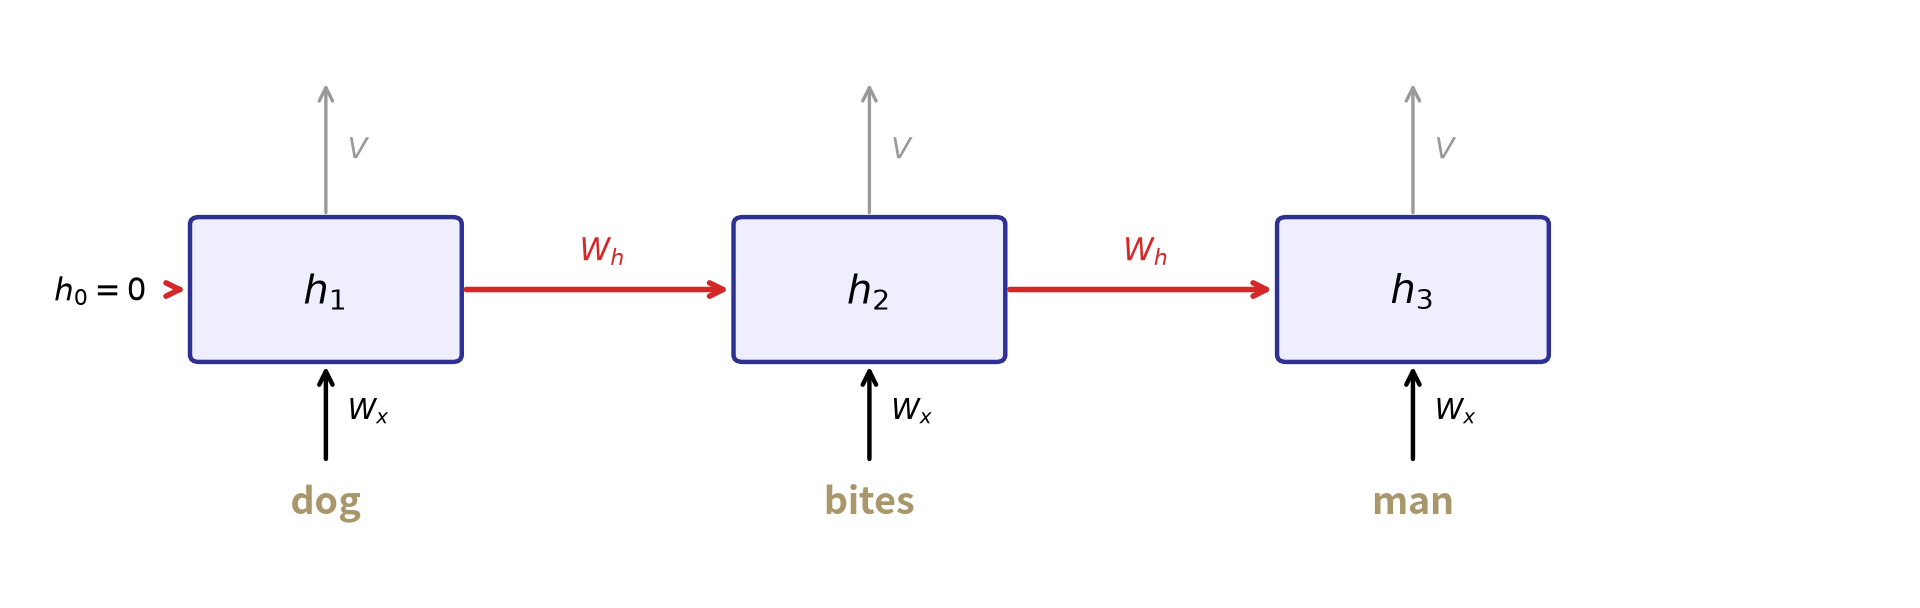
\includegraphics[width=0.9\linewidth]{rn_unroll.png}\par\vskip0.2em
{\large 메모가 \textcolor{ksared}{$W_h$} 를 타고 다음 단어로 넘어간다 \quad 마지막 메모 $\mathbf{h}_3$ 에 문장 전체가 담긴다}
\vfill
\note{RNN을 시간 순서대로 펼쳐 그리면 이렇습니다. 첫 단어 dog을 읽어 메모 h1을 만들고, 이 메모가 빨간 W_h를 타고 다음 칸으로 넘어가 bites와 합쳐져 h2가 되고, 다시 man과 합쳐져 h3가 됩니다. 마지막 메모 h3에는 문장 전체를 순서대로 읽은 결과가 담깁니다. 펼친 그림은 깊은 신경망처럼 보이지만, 모든 칸의 가중치는 같습니다.}
\end{frame}

% --- 손 계산
\begin{frame}{손으로 한 번: 메모가 한 칸인 RNN}
\vfill
\centering
{\large $h_t = \tanh(1 \cdot x_t + 0.5 \cdot h_{t-1})$, \quad 입력 $x = 1, 0, 1$}\vskip0.6em
\renewcommand{\arraystretch}{1.5}
{\Large\begin{tabular}{lll}
$t = 1$ & $\tanh(1 + 0.5 \times 0)$ & $= 0.762$\\
$t = 2$ & $\tanh(0 + 0.5 \times 0.762) = \tanh(0.381)$ & $= 0.363$\\
$t = 3$ & $\tanh(1 + 0.5 \times 0.363) = \tanh(1.182)$ & $= \kb{0.828}$
\end{tabular}}\vskip0.6em
{\large 입력이 0 인 둘째 칸에서도 메모는 0 이 아니다 \quad \textbf{앞의 1 을 기억}하고 있다}
\vfill
\note{메모가 한 칸뿐인 RNN으로 직접 계산해 봅니다. 가중치는 입력에 1, 이전 메모에 0.5입니다. 입력은 1, 0, 1입니다. 첫째 칸은 tanh 1, 0.762입니다. 둘째 칸은 입력이 0이지만 이전 메모의 절반 0.381이 들어와 tanh를 씌우면 0.363입니다. 입력이 없어도 앞에서 본 1을 기억하고 있는 겁니다. 셋째 칸은 입력 1에 이전 메모의 절반을 더한 1.182, tanh를 씌워 0.828입니다. 만약 입력이 0, 1, 1이었다면 마지막 메모는 달라집니다. 순서가 메모에 남습니다.}
\end{frame}

% --- 두 문장
\begin{frame}{두 문장의 마지막 메모는 다르다}
\markpage{memo}
\vfill
\centering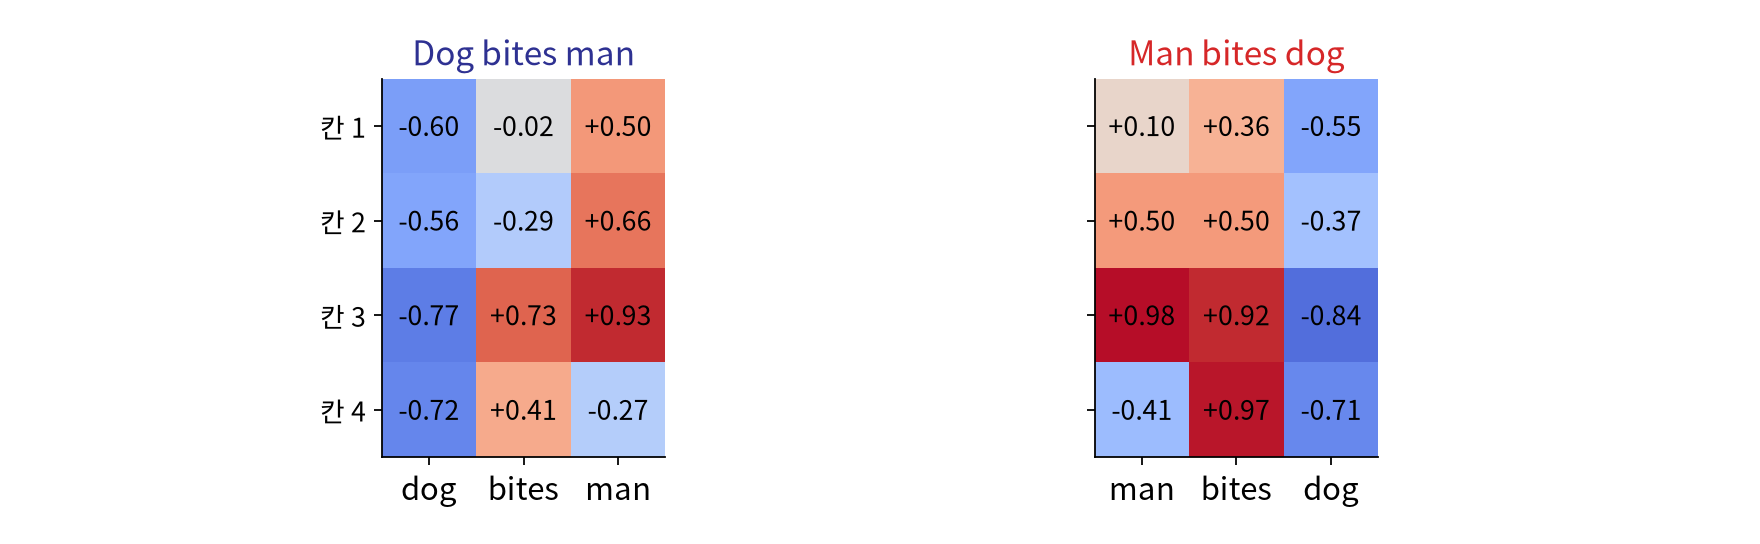
\includegraphics[width=0.92\linewidth]{rn_memo.png}\par\vskip0.2em
{\large 마지막 메모: \kb{$(+0.50, +0.66, +0.93, -0.27)$} vs \kq{$(-0.55, -0.37, -0.84, -0.71)$}}\\[0.2em]
{\small 같은 RNN (메모 4칸, 학습 전 무작위 가중치) \quad 학습은 이 메모가 \textbf{뜻}을 담도록 고친다}
\vfill
\note{메모가 4칸인 RNN에 두 문장을 넣어 봤습니다. 가중치는 학습 전의 무작위 값입니다. 같은 단어 세 개를 읽었지만, 순서가 다르니 단계마다 메모가 다르고, 마지막 메모는 플러스 0.5, 0.66, 0.93, 마이너스 0.27과 마이너스 0.55, 0.37, 0.84, 0.71로 완전히 다릅니다. 덧셈과 달리 순서를 구별합니다. 학습은 이 마지막 메모가 누가 누구를 물었는지 같은 뜻을 잘 담도록 가중치를 고치는 과정입니다.}
\end{frame}

\section{언어 모델}
% --- 언어 모델
\begin{frame}{RNN 언어 모델: 다음 글자 맞히기}
\vfill
\centering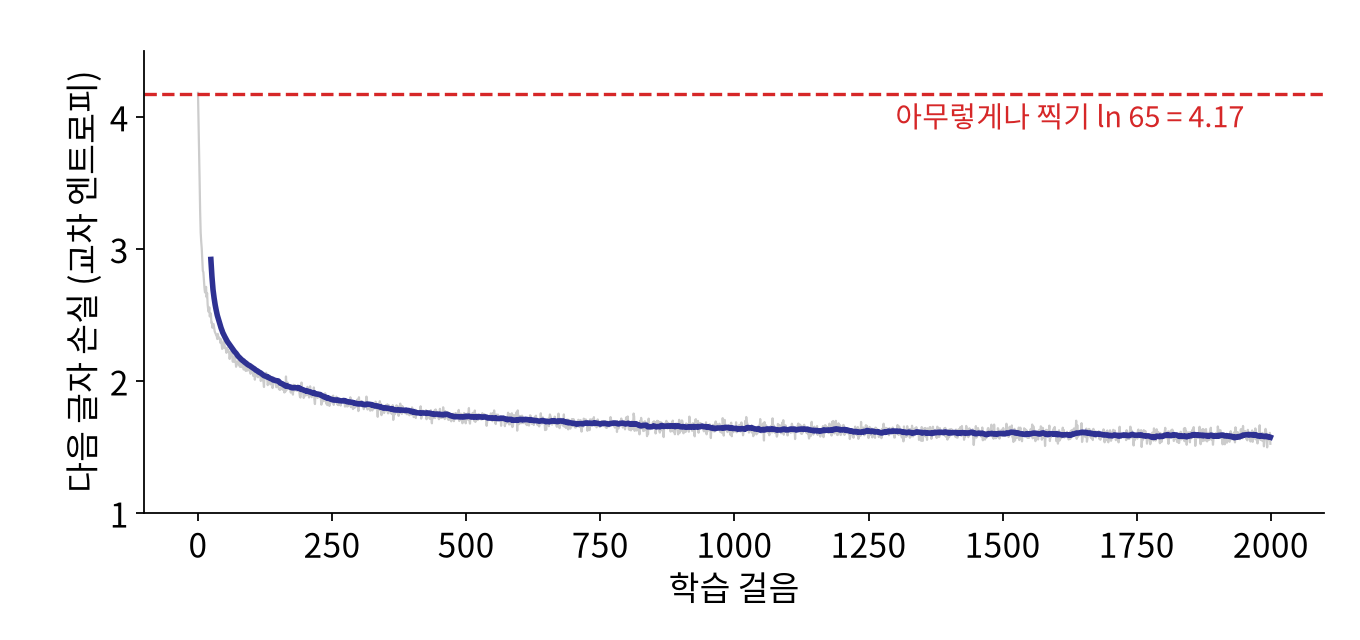
\includegraphics[width=0.56\linewidth]{rn_loss.png}\par\vskip0.2em
{\large 셰익스피어 희곡 111만 글자, 매 칸에서 \textbf{다음 글자}를 맞히도록 학습 (교차 엔트로피)}\\[0.2em]
{\large 손실: 처음 4.18 (찍기 수준) $\to$ 2,000걸음 뒤 \kb{1.58}}
\vfill
\note{RNN으로 언어 모델을 만들어 봤습니다. 셰익스피어 희곡 111만 글자로, 매 칸에서 다음 글자를 맞히도록 학습했습니다. 출력 V h_t가 65가지 글자의 점수이고, 손실은 2주차의 교차 엔트로피입니다. 처음 손실은 4.18로, 65가지를 아무렇게나 찍을 때의 ln 65, 4.17과 같습니다. 2000걸음 학습하면 1.58까지 내려갑니다.}
\end{frame}

% --- 생성
\begin{frame}{학습한 RNN 이 쓴 글}
\vfill
\centering
\renewcommand{\arraystretch}{1.3}
{\small\begin{tabular}{p{0.12\linewidth}p{0.8\linewidth}}
\textbf{200걸음} & \texttt{ROMEO: Why mome kish selled ouch me hand, in I to the My course his thee reching thin bein so mane him stints, your well deatces is dinger not my fits,}\\[0.6em]
\textbf{2,000걸음} & \texttt{ROMEO: Why make it with the death expenty in I the can you upon him thee reshian of bloodel some shall stants, your way, and come are forrone; my father we would for me I see they ches of the wife, sir.}
\end{tabular}}\vskip0.8em
{\large 다음 글자를 뽑아 다시 넣기를 반복 \quad 단어 · 띄어쓰기 · 구두점을 배웠다}\\[0.2em]
{\small 뜻은 아직 엉망 \quad 은닉 128칸 RNN, 몇 분 학습 (Karpathy char-rnn 을 작게 재현)}
\vfill
\note{학습한 RNN에게 ROMEO 콜론을 주고, 다음 글자를 뽑아 다시 넣기를 200번 반복했습니다. 200걸음만 학습했을 때는 단어 비슷한 것이 나오지만 대부분 틀린 철자입니다. 2000걸음 뒤에는 make, death, father, wife, sir 같은 진짜 단어가 많아지고, 띄어쓰기와 쉼표, 세미콜론, 마침표도 그럴듯하게 씁니다. 뜻은 아직 엉망이지만, 글자 단위로 읽는 작은 RNN이 몇 분 만에 영어의 모양을 배운 겁니다. 2015년 카파시의 char-rnn 실험을 작게 재현한 것입니다.}
\end{frame}

\section{학습 · 약점}
% --- BPTT
\begin{frame}{학습: 시간을 거슬러 역전파 (BPTT)}
\vfill
\centering
{\large 펼친 그림 \pref{unroll} 에서 역전파 \quad 같은 가중치의 \textbf{기울기를 칸마다 더한다}}\vskip0.6em
{\LARGE\[ \frac{\partial L}{\partial \mathbf{h}_1} = \frac{\partial L}{\partial \mathbf{h}_T}\;\prod_{t=2}^{T} \frac{\partial \mathbf{h}_t}{\partial \mathbf{h}_{t-1}} \]}\vskip0.2em
{\large 오래전 단어로 가는 기울기는 \textbf{여러 번 곱해진다} $\to$ \kq{기울기 소실} (7주차)}
\vfill
\note{학습은 펼친 그림에서 그대로 역전파를 합니다. 시간을 거슬러 올라가는 역전파, BPTT라고 부릅니다. 같은 가중치가 여러 칸에 쓰였으니 칸마다 구한 기울기를 모두 더합니다. 문제는 오래전 단어로 가는 기울기입니다. 마지막 메모에서 첫 메모까지 가려면 W_h와 tanh의 기울기를 칸 수만큼 곱해야 합니다. 7주차에 깊은 신경망에서 봤던 기울기 소실이 여기서는 시간 방향으로 일어납니다.}
\end{frame}

% --- 기억 감쇠
\begin{frame}{약점: 오래된 기억이 흐려진다}
\vfill
\centering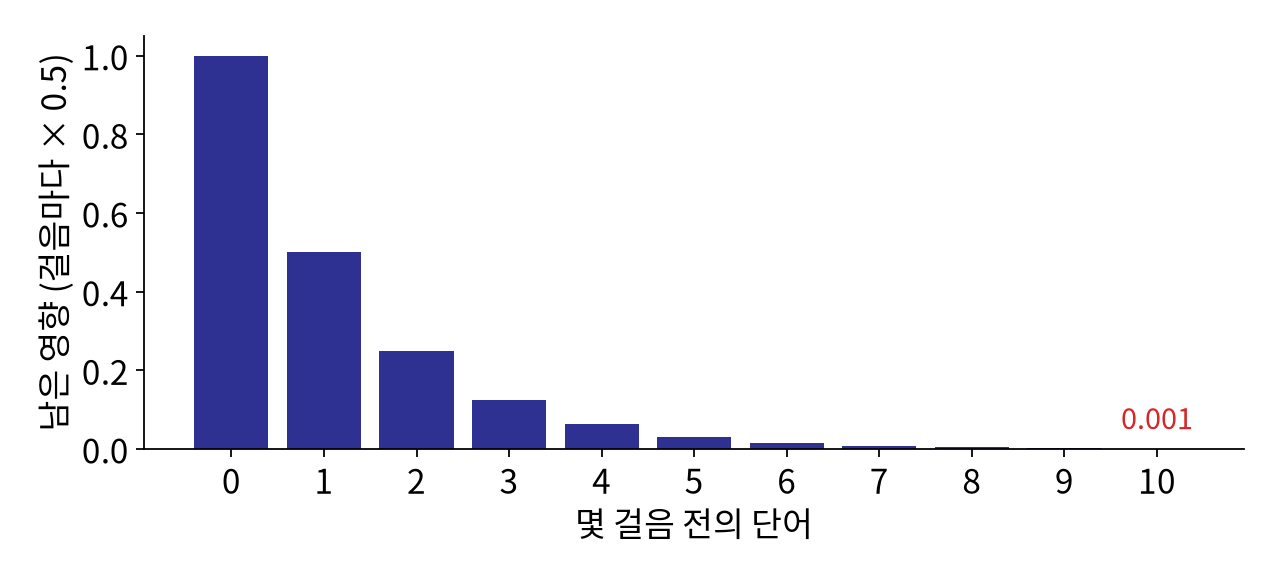
\includegraphics[width=0.56\linewidth]{rn_decay.png}\par\vskip0.2em
{\large 한 걸음마다 영향이 절반으로 준다면 \quad 10걸음 뒤 $0.5^{10} \approx \kq{0.001}$}\\[0.2em]
{\small ``The \textbf{cat}, which ate all the fish in the kitchen, \textbf{was} full'': 멀리 떨어진 cat 과 was}
\vfill
\note{그래서 기본 RNN은 오래된 기억이 흐려집니다. 예를 들어 한 걸음마다 영향이 절반으로 줄어든다면 10걸음 뒤에는 0.001배만 남습니다. 학습할 때도 멀리 떨어진 단어 사이의 관계를 배우기 어렵습니다. The cat, which ate all the fish in the kitchen, was full이라는 문장에서 was가 단수인 이유는 한참 앞의 cat 때문인데, 둘 사이가 멀면 RNN이 이 연결을 배우기 힘듭니다. 다음 시간에 이 문제를 기억 통로로 해결한 LSTM을 배웁니다.}
\end{frame}

% --- 쓰임
\begin{frame}{RNN 이 쓰인 곳}
\vfill
\centering
\renewcommand{\arraystretch}{1.5}
{\large\begin{tabular}{lll}
\textbf{여러 개 $\to$ 하나} & 문장 $\to$ 감정 (긍정 / 부정) & 마지막 메모로 분류\\
\textbf{여러 개 $\to$ 여러 개} & 다음 글자 · 단어 예측, 품사 붙이기 & 칸마다 출력\\
\textbf{입력 $\to$ 다른 길이 출력} & 번역 (11주차 Seq2Seq) & 읽는 RNN + 쓰는 RNN
\end{tabular}}\vskip0.8em
{\small 2017년 트랜스포머 이전, 번역 · 음성 인식의 주력 \quad 지금도 작은 시계열 · 실시간 처리에 쓰인다}
\vfill
\note{RNN은 이렇게 쓰입니다. 문장을 다 읽고 마지막 메모로 긍정, 부정을 가리는 것처럼 여러 개를 읽고 하나를 내는 경우, 오늘처럼 칸마다 다음 글자를 내는 경우, 그리고 11주차에 배울 번역처럼 읽는 RNN과 쓰는 RNN을 이어 붙이는 경우가 있습니다. 2017년 트랜스포머가 나오기 전까지 번역과 음성 인식의 주력이었고, 지금도 작은 시계열이나 실시간 처리에 쓰입니다.}
\end{frame}

\section{연습}
% --- 문제풀이
\begin{frame}{문제풀이}
\vfill
\begin{enumerate}
\item 손 계산 예 ($w_x = 1$, $w_h = 0.5$) 에 입력 $0, 1, 1$ 을 넣으면 $h_1, h_2, h_3$ 는? ($\tanh 1 = 0.762$, $\tanh 1.381 = 0.881$)\vskip0.8em
\item 단어 벡터 100칸, 메모 200칸인 RNN 의 $W_x$, $W_h$, $\mathbf{b}$ 가중치 수는? 문장이 길어지면 가중치 수는?\vskip0.8em
\item 글자 65가지에서 아무렇게나 찍을 때의 교차 엔트로피는 왜 $\ln 65$ 인가?\vskip0.8em
\item 한 걸음마다 기억이 0.8 배가 된다면 20걸음 뒤에는? ($0.8^{10} \approx 0.107$)
\end{enumerate}
\vfill
\note{1번 답. h1은 tanh 0, 0입니다. h2는 tanh 1, 0.762, h3는 tanh 1 더하기 0.381, tanh 1.381, 0.881입니다. 2번 답. W_x는 200 곱하기 100, 2만, W_h는 200 곱하기 200, 4만, b는 200, 합쳐 6만 200개입니다. 문장이 길어져도 그대로입니다. 3번 답. 모든 글자에 65분의 1을 주면 정답 글자의 확률이 65분의 1이라 마이너스 ln 65분의 1, ln 65입니다. 4번 답. 0.107의 제곱, 약 0.011입니다.}
\end{frame}

% --- 실습
\begin{frame}{실습}
\vfill
\centering\begin{tabular}{rl}
\large 1 & numpy 로 RNN 한 칸 구현 $\to$ 손 계산 0.762 · 0.363 · 0.828, 두 문장의 메모 비교\\[0.5em]
\large 2 & PyTorch \texttt{nn.RNN} 으로 글자 단위 언어 모델 (셰익스피어)\\[0.5em]
\large 3 & 학습 중간중간 글 써 보기, 온도 바꿔 보기
\end{tabular}\vskip1em
Tiny Shakespeare (Karpathy, char-rnn) \\[0.4em]\href{https://colab.research.google.com/github/SuminHan/book-ml/blob/main/slides/v2/ml1/week11/rnn/lab/rnn.ipynb}{\textcolor{ksagolddk}{▶ Colab에서 실습 노트북 열기}}
\vfill
\note{실습은 세 부분입니다. 첫째, numpy로 RNN 한 칸을 구현해서 손 계산을 재현하고, 두 문장의 메모를 비교합니다. 둘째, PyTorch의 nn.RNN으로 셰익스피어 글자 단위 언어 모델을 만들어 학습합니다. 셋째, 학습 중간중간 글을 써 보고, 온도를 바꾸면 글이 어떻게 달라지는지 봅니다.}
\end{frame}

\section{정리}
% --- 정리
\begin{frame}{정리}
\vfill
\centering\large\begin{tabular}{l}
순서가 중요한 데이터: 단어를 더하면 순서를 잃는다\\[0.5em]
\textbf{RNN} \quad $\mathbf{h}_t = \tanh(W_x \mathbf{x}_t + W_h \mathbf{h}_{t-1} + \mathbf{b})$ \quad 모든 칸에서 같은 가중치\\[0.5em]
언어 모델: 다음 글자 맞히기, 손실 4.18 $\to$ 1.58, 영어 모양을 배운다\\[0.5em]
BPTT 에서 곱셈이 쌓여 \kq{오래된 기억이 흐려진다} $\to$ 다음 시간 LSTM
\end{tabular}
\vfill
\note{정리합니다. 문장처럼 순서가 중요한 데이터는 단어를 그냥 더하면 순서를 잃습니다. RNN은 단어를 하나씩 읽으며 은닉 상태라는 메모를 고쳐 쓰고, 모든 칸에서 같은 가중치를 씁니다. 다음 글자를 맞히는 언어 모델로 학습하면 손실이 4.18에서 1.58로 내려가며 영어의 모양을 배웁니다. 다만 시간을 거슬러 역전파할 때 곱셈이 쌓여 오래된 기억이 흐려지고, 다음 시간 LSTM이 이 문제를 해결합니다.}
\end{frame}
\end{document}
